\documentclass[12pt]{report}
\usepackage{amssymb,amsmath}
\usepackage[utf8]{inputenc}
\usepackage[spanish]{babel}
\selectlanguage{spanish}
\usepackage{graphicx}
\usepackage{pgfplots}
\usepackage{tikz}
\usepackage{enumerate}
\usepackage{listings}
\usepackage{multirow} % para las tablas
\usepackage[T1]{fontenc}
\usepackage{mathrsfs} 
\usepackage{multirow} % para las tablas
\lstset{language=Matlab, breaklines=true, basicstyle=\footnotesize}
\lstset{numbers=left, numberstyle=\tiny, stepnumber=1, numbersep=-8pt}

%%formato de leonel 
\setlength{\voffset}{0pt}

\setlength{\topmargin}{-32pt}
\setlength{\headheight}{20pt}
\setlength{\headsep}{19pt}
\setlength{\topskip}{0pt}
\setlength{\oddsidemargin}{0pt}
\setlength{\evensidemargin}{0pt}
\setlength{\marginparwidth}{0.75in}
\setlength{\marginparsep}{0.1in}

\setlength{\abovecaptionskip}{3pt}
\setlength{\footskip}{30pt}

\setlength{\textwidth}{\paperwidth}
\addtolength{\textwidth}{-2in}
\setlength{\textheight}{\paperheight}
\addtolength{\textheight}{-1.75in}

\setlength{\parindent}{1em}
\setlength{\parskip}{0.3em}
%%leonel

\begin{document}
\tableofcontents
%%portada
\begin{titlepage}
%%portada
		\begin{center}
			\vspace*{-1in}
			\begin{figure}[htb]
			\centering
					
\includegraphics[scale=0.2]{logo_original}
			\end{figure}
			
			TECNOLÓGICO NACIONAL DE MÉXICO\\
			\vspace*{0.15in}
			INSTITUTO TECNOLÓGICO DE MORELIA \\
			\vspace*{0.3in}
			\begin{large}
				DEPARTAMENTO DE INGENIERÍA ELECTRÓNICA\\
			\end{large}
			\vspace*{0.2in}
			\begin{large}
				Control 1\\
			\end{large}
		\vspace*{0.3in}
			\begin{Large}
				\textbf{Práctica 2\\
				Encontrar por Inspección los Polos y Ceros} \\
			\end{Large}
			\vspace*{0.3in}
			\begin{large}
			Profesor:Gerardo Marx Chávez Campos\\
			\end{large}
			\vspace*{0.2in}
		\begin{large}
			Alumnos : \\
			Carlos Ivan Ramírez Arguello\\
			Edrei Martinez Lopez\\
		\end{large}
			\vspace*{0.3in}
			\rule{80mm}{0.1mm}\\
			\vspace*{0.1in}
			\begin{large}
				MORELIA, MICHOACÁN \\
				Fecha de Entrega:\\
				01/diciembre/2017 \\
			\end{large}
		\end{center}
	\end{titlepage}
%%portada
%%reporte
\chapter{Introducción}
 FUNCIONES DE TRANSFERENCIA\\
Una de las herramientas más importantes de la representación entrada-salida es la
función de transferencia. La idea de emplear funciones de transferencia para
representar sistemas físicos es una consecuencia natural del uso de la transformada de
Laplace para resolver ecuaciones diferenciales lineales. Resulta razonable que estos
métodos tengan un gran valor en la representación de sistemas, ya que han resultado
sumamente exitosos en la simplificación y sistematización del problema que se presenta
para obtener la respuesta en el tiempo de un sistema.\\
La configuración general de un sistema de control en lazo cerrado, el cual esta formado por dos elementos básicos: la planta y el controlador.
La planta comprende la parte inalterable del sistema. Para obtener un desempeño
adecuado del sistema global, el diseñador añade el controlador. Para comprender como se
emplean las funciones de transferencia en la representación de la planta, supóngase que
si se tiene una planta general de n-ésimo orden, con una entrada de control u(t) y una
salida y(t).\\
Esta ecuación diferencial proporciona una descripción completa de la planta, en el
sentido de que se puede determinar la salida cualesquiera que sean las condiciones
iniciales y la entrada. En realidad, la ecuación diferencial, ya es un modelo matemático
que sólo se aproxima al comportamiento de la planta física. No obstante, este modelo es
poco manejable y por ende, rara vez se le emplea de esta forma.
 El conjunto de ecuaciones diferenciales que describen las leyes físicas que
determinan el comportamiento de los componentes individuales de la planta es el punto de
partida básica. [1]

\chapter{Metodología}
Se realizan los cálculos por inspección y algebraico partiendo de una función de transferencia del circuito para poder realizar una buen análisis como se muestra en los siguientes cálculos así encontrar cuales son los dispositivos que pueden llevar a el circuito a tener un mal funcionamiento ó inestabilidad o estabilidad.
\section{Parte 1}
\subsection{Cálculos}
\subsubsection{Algebraico}
\begin{equation*}
R_{eq}=(R_2+SL)\parallel R_3=\frac{R_2+SL}{R_2+SL+R3}
\end{equation*}
\begin{equation*}
\frac{R_2R_3+R_3SL}{R_2+SL+R_3}
\end{equation*}
\begin{equation*}
V_{out}=V_{in}\frac{\frac{R_2R_3+R_3SL}{R_2+SL+R_3}}{R_1+\frac{R_2R_3+R_3SL}{R_2+SL+R_3}}
\end{equation*}
\begin{equation*}
\frac{V_{out}}{v_{in}}=\frac{\frac{R_2R_3+R_3SL}{R_2+SL+R_3}}{\frac{R_1(R_1+SL+R_3)+R_2R_3+R_3SL}{R_2+SL+R_3}}
\end{equation*}
\begin{equation*}
\frac{V_{out}}{v_{in}}=\frac{R_2R_3+R_3SL}{R_1(R_1+SL+R_3)+R_2R_3+R_3SL}
\end{equation*}
\begin{equation*}
\frac{V_{out}}{v_{in}}=\frac{R_2R_3+R_3SL}{R_1R_2+R_1SL+R_1R_3+R_2R_3+R_3SL}
\end{equation*}
\begin{equation*}
\frac{V_{out}}{v_{in}}=\frac{R_3(R_2+SL)}{R_1R_2+R_1R_3+R_2R_3+R_1SL+R_3}
\end{equation*}
\begin{equation*}
\frac{V_{out}}{v_{in}}=\frac{R_3SL+R_3R_2}{(R_1R_2+R_1R_3+R_2R_3)+R_1SL+R_3SL}
\end{equation*}
\begin{equation*}
\frac{V_{out}}{v_{in}}=\frac{R_2R_3(\frac{SL}{R_2}+1)}{R_1(R_2+R_3)+R_2R_3(1+\frac{SL(R_1+R_3)}{R_1(R_2R_3)+R_2R_1}}
\end{equation*}
\begin{equation*}
\frac{V_{out}}{v_{in}}=(\frac{R_2 \parallel R_3}{R_1+R_2 \parallel R_3})(\frac{\frac{SL}{R_2}+1}{1+\frac{SL(R_1+R_3)}{R_1R_2+R_3+R_1+R_2R_3}})
\end{equation*}
\begin{equation*}
\frac{V_{out}}{v_{in}}=(\frac{R_2 \parallel R_3}{R_1+R_2 \parallel R_3})(\frac{\frac{SL}{R_2}+1}{1+\frac{SL(R_1+R_3)}{R_1R_3+R_2(R_1+R_3)}})
\end{equation*}
\begin{equation*}
\frac{V_{out}}{v_{in}}=(\frac{R_2 \parallel R_3}{R_1+R_2 \parallel R_3})(\frac{\frac{SL}{R_2}+1}{1+\frac{SL(R_1+R_3)}{(R_1+R_3)(\frac{R_1R_3}{R_1+R_3}+R_2)}})
\end{equation*}
\begin{equation*}
\frac{V_{out}}{v_{in}}=(\frac{R_2 \parallel R_3}{R_1+R_2 \parallel R_3})(\frac{\frac{SL}{R_2}+1}{1+\frac{SL}{R_1\parallel R_3+R_2}})
\end{equation*}

\subsubsection{Inspección}
1.-Forma de la función de transferencia 
\begin{figure}[h!]
  \centering
    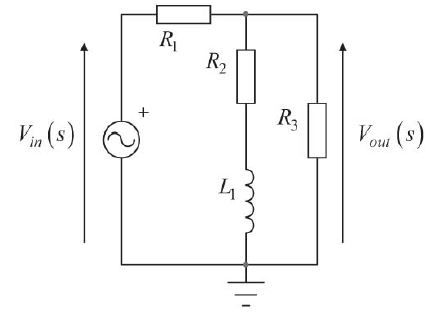
\includegraphics[width=3.5in]{parte1}
  \caption{Circuito abierto en la rama que afecta  para sacar los polos.}
\end{figure}
\begin{equation}
V_{out}=V_{in}(\frac{R_2 \parallel R_3}{R_2 \parallel R_3+R_1})
\end{equation}
\begin{equation*}
\frac{ V_{out}}{V_{in}}=(\frac{R_2 \parallel R_3}{R_2 \parallel R_3+R_1})=H(s)
\end{equation*}
2.- Zero = cero la rama que afecta el circuito.
\begin{equation*}
R_2+SL=0
\end{equation*}
\begin{equation*}
\frac{R_2}{R_2}+\frac{SL}{R_2}=\frac{1}{R_2}
\end{equation*}
\begin{equation*}
1+\frac{SL}{R_2}=0
\end{equation*}
\begin{equation*}
1+\frac{S}{W_{Z1}}=0
\end{equation*}
\begin{equation*}
W_{Z1}=\frac{R_2}{L}
\end{equation*}
\begin{equation*}
1+\frac{SL}{R_2}=1+\frac{S}{W_{Z1}}
\end{equation*}
\begin{equation*}
\frac{SL}{R_2}=\frac{S}{W_Z1} \rightarrow  W_Z1=\frac{SR_2}{SL}=\frac{R_2}{L}
\end{equation*}
3.- En el siguiente paso sacaremos los polos para los estados de nuestro circuito.  
\begin{figure}[h!]
  \centering
    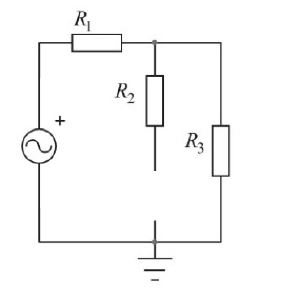
\includegraphics[width=2.5in]{parte3}
  \caption{Circuito abierto en la rama que afecta  para sacar los polos.}
\end{figure}
\begin{equation*}
R_{eq}=R_2+R_1 \parallel R_3
\end{equation*}
\begin{equation*}
\tau=\frac{L}{R_{eq}} \rightarrow W_P1=\frac{L}{R_{eq}}= W_P1=\frac{L}{R_2+R_1 \parallel R_3}
\end{equation*}
\begin{equation*}
W_P2=\frac{1}{\tau}=\frac{1}{\frac{L}{R_{eq}}}=\frac{R_2+R_1 \parallel R_3}{L}
\end{equation*}
\section{Parte 2}
\begin{figure}[h!]
  \centering
    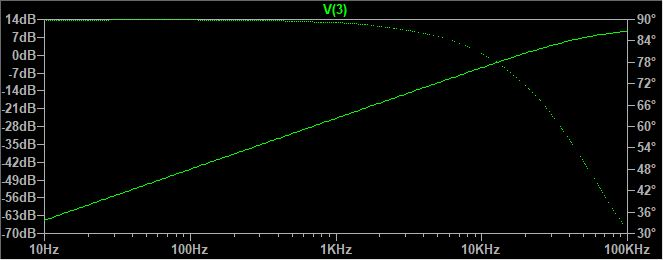
\includegraphics[width=3.5in]{ac}
  \caption{Respuesta del circuito como filtro pasa altas.}
\end{figure}
\begin{lstlisting}[frame=single]
    Vin 1 0 AC 5
    R1 1 2 1k
    R2 2 3 330
    R3 2 0 2.20k
    L1 3 0 2.7mH
    .ac dec 10  10H 100k
    .end

\end{lstlisting}
\begin{figure}[h!]
  \centering
    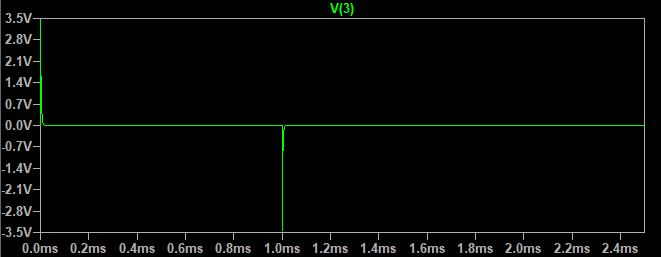
\includegraphics[width=3.5in]{pulse}
  \caption{Transitorio.}
\end{figure}
\begin{figure}[h!]
  \centering
    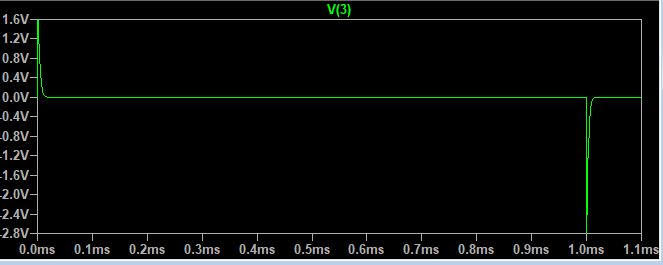
\includegraphics[width=3.5in]{pulse2}
  \caption{Transitorio del circuito con funciòn impulso.}
\end{figure}
\begin{lstlisting}[frame=single]
    Vin  1 0   pulse(0v,5v,0s,1ns,1ns,1ms,2ms,3ms,4ms,5ms) 
    R1 1  2  1k
    R2 2  3  330
    R3 2  0  2.2k
    L1 3 0    2.7mH
    .tran     100us   2.5ms
    .end
\end{lstlisting}
Silab:
\begin{lstlisting}[frame=single]
    s =%s
    poly (0 , 's')
    wz1=122222.2222;
    wp1=0.000002653;
    wp2=376851.8519;
    simpleSys=syslin('c', wz1/((s/wp1)+(s/wp2))) //funcio de        transferencia
    t=0:0.0001:100000;
    y=csim('step', t, simpleSys)//funcion escalon step
    plot(t,y)
    xlabel('frecuencia (Hz)')
    ylabel('decibeles(dB)')
\end{lstlisting}
\begin{figure}[h!]
  \centering
    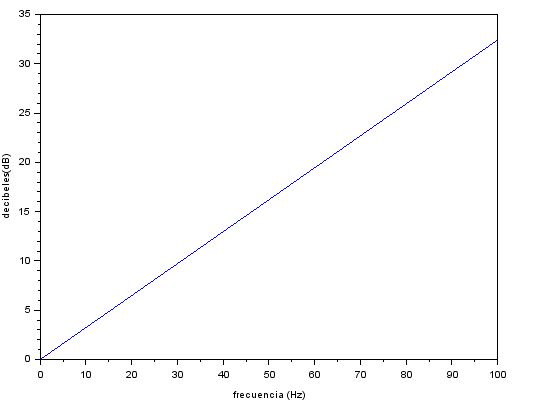
\includegraphics[width=3.5in]{silabimag}
  \caption{Ecuacion en Silab.}
\end{figure}
\section{Parte 3}
Barrido de dato en frecuencia:\\
Se hace un barrido en frecuencia en el cual nos muestra el funcionamiento del dispositivo el cual nos arroja como resultado el análisis espectral nos hace ver que el circuito tiene frecuencias de corte por que se ingresa una señal la cual tiene un ancho de banda de trabajo así como a mayoría de los componentes de silicio tienen problemas con la frecuencia hay puntos en bajas frecuencias en las que atenúan y al aumentar la frecuencia sube la amplitud pero  al ir aumentando sigue pasando este mismo funcionamiento en la salida atenúa a alguna frecuencia y sufre un aumento de amplitud el cual esta registrado en la siguiente tabla.\\
\begin{table}[htbp]
\begin{center}
\begin{tabular}{|l|l|}
\hline
Voltaje & Frecuencia \\
\hline \hline
0.92  & 10\\ \hline
1.08  & 20\\ \hline
1.08  & 30 \\ \hline
1.08  & 40\\ \hline
1.12  & 50 \\ \hline
1.12  & 60 \\ \hline
1.12  & 70 \\ \hline
1.12  & 80 \\ \hline
1.12  & 90 \\ \hline
1.12  & 1000 \\ \hline
1.12  & 2000 \\ \hline
1.12  & 3000 \\ \hline
1.12  & 4000\\ \hline
1.12  & 5000 \\ \hline
1.12  & 6000 \\ \hline
1.12  & 7000 \\ \hline
1.12  & 8000 \\ \hline
1.12  & 9000\\ \hline
2.36  & 1000000 \\ \hline
1.84  & 1500000 \\ \hline
1.6   & 2000000 \\ \hline
\end{tabular}
\caption{Tabla de barrido en frecuencia con el generador de funciones.}

\label{tabla:sencilla}
\end{center}
\end{table}
Comportamiento gráficamente de los valores medidos del circuito en la practica son los siguiente:\\
\begin{figure}[h!]
  \centering
    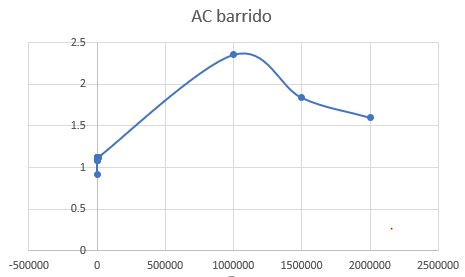
\includegraphics[width=3.5in]{barrido}
  \caption{gráfica de barrido.}
  \end{figure}
  \begin{figure}[h!]
  \centering
    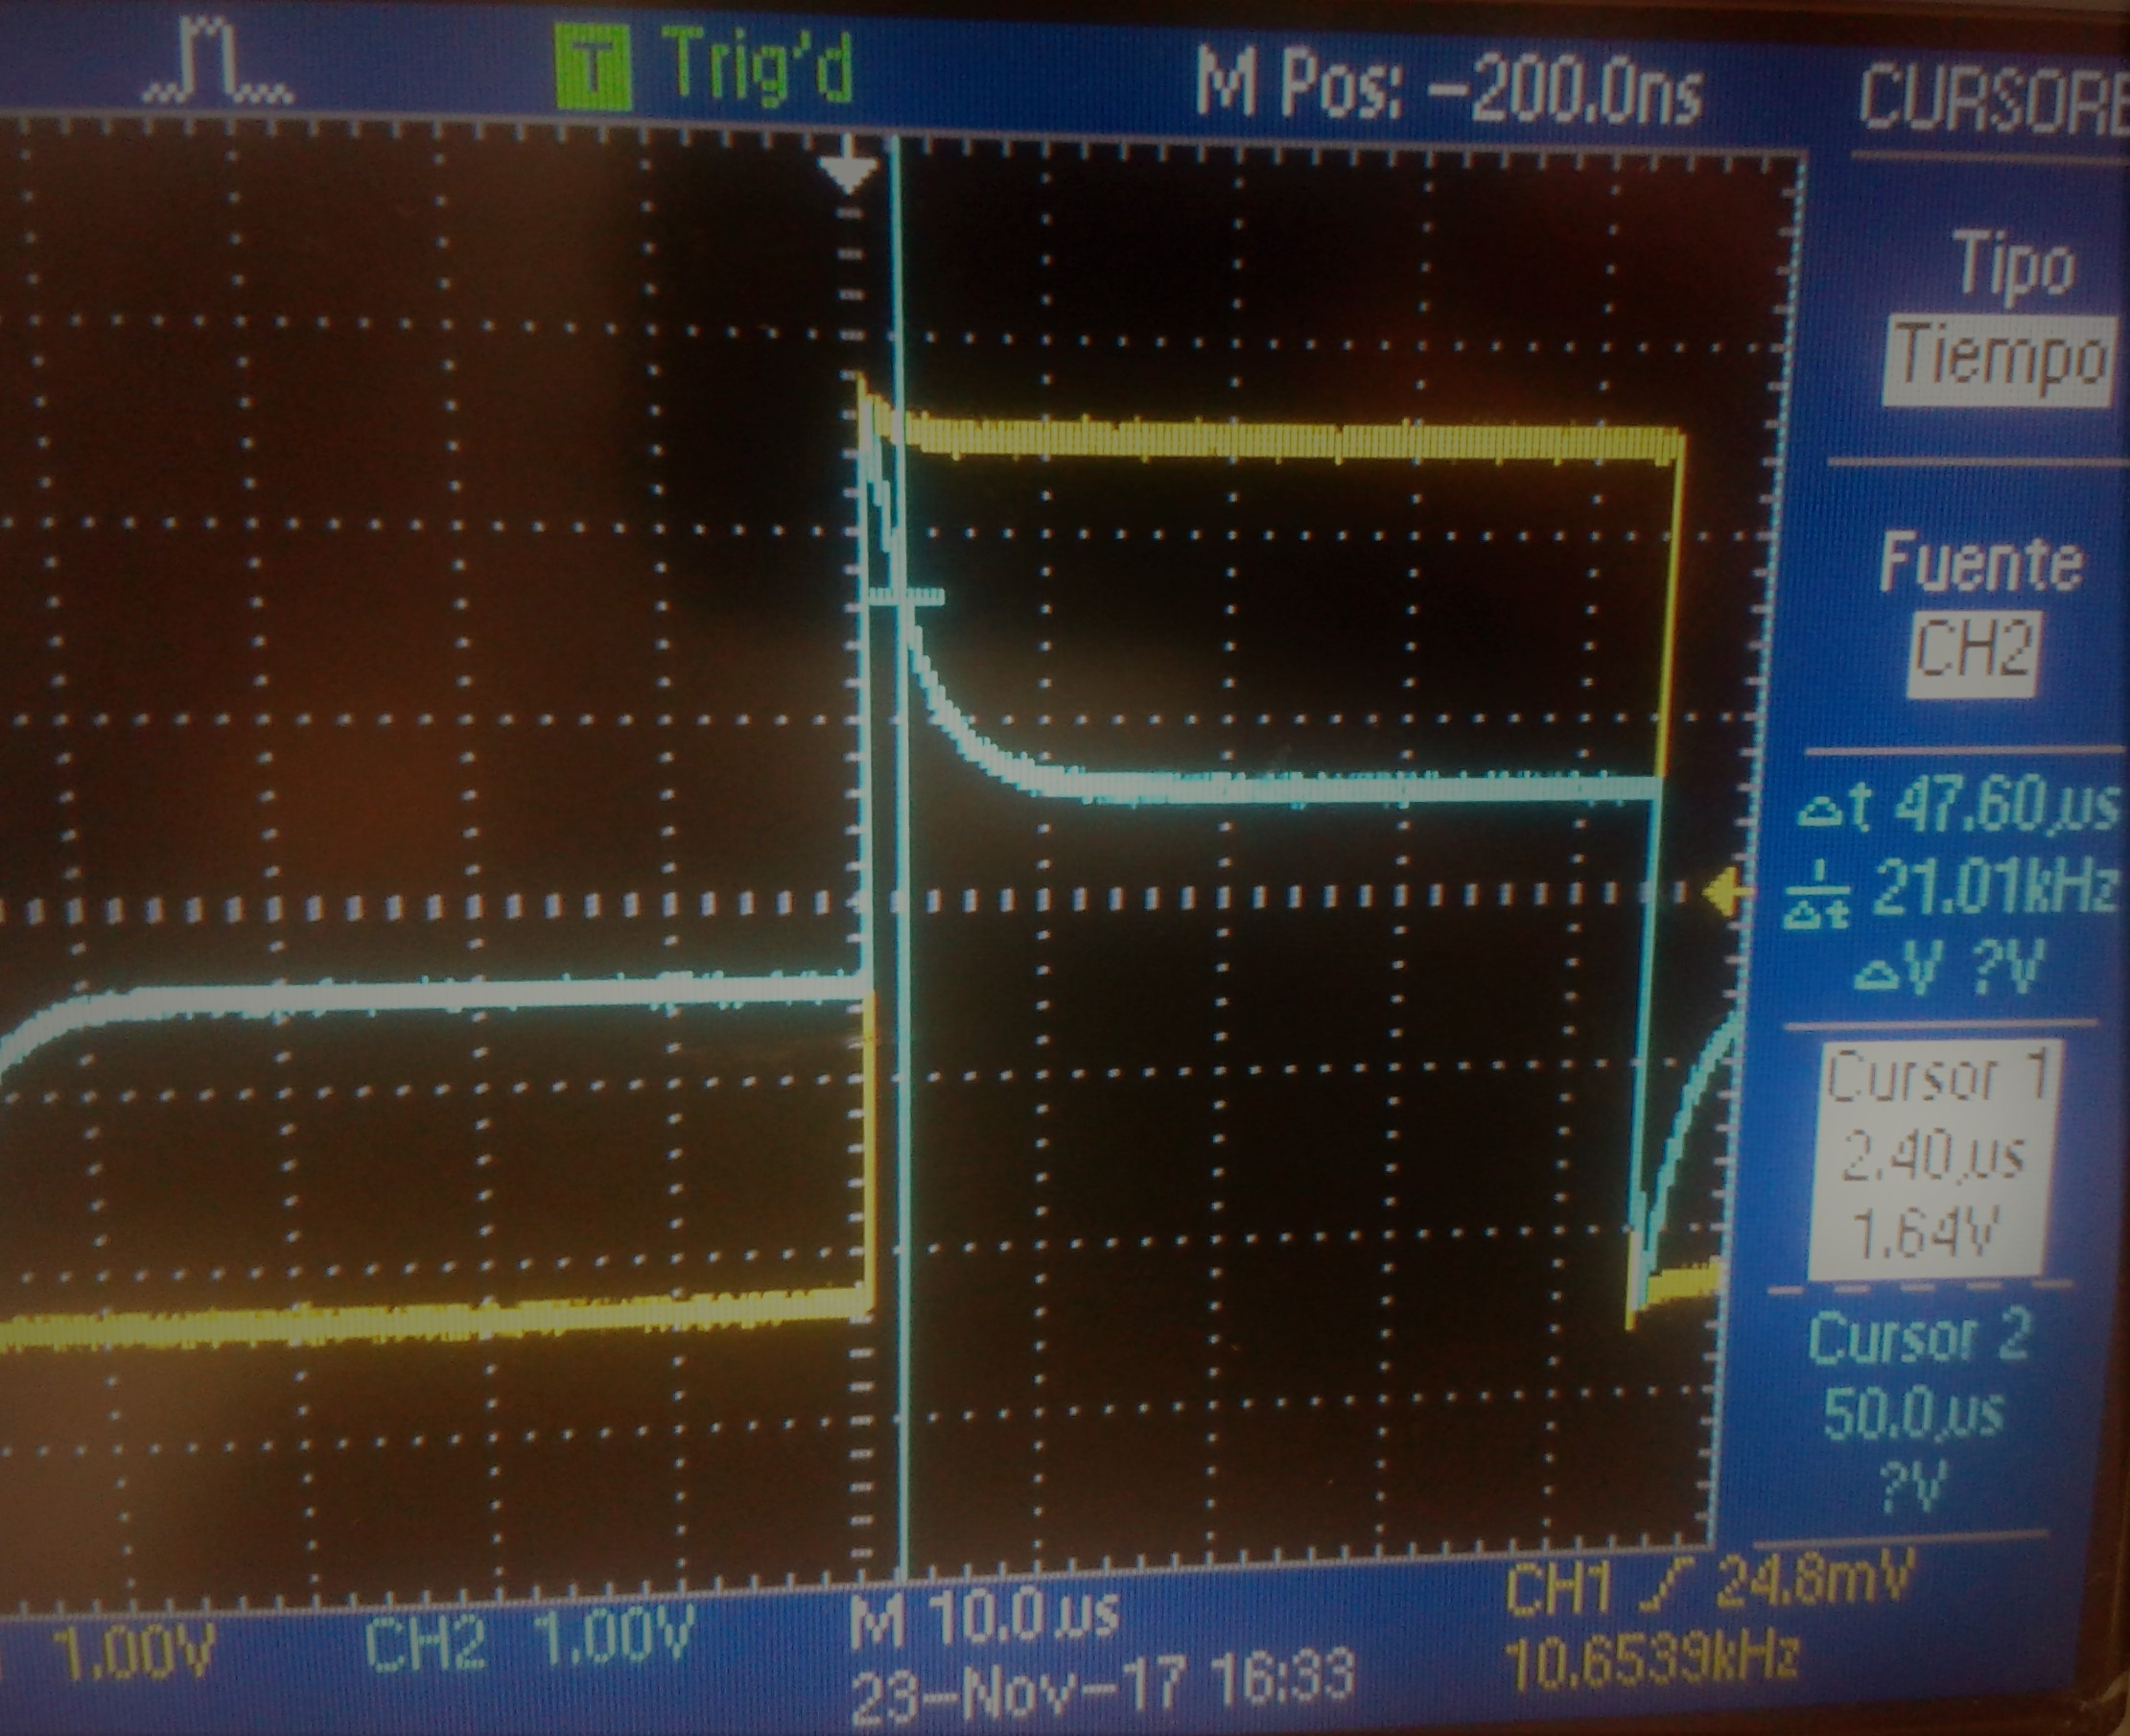
\includegraphics[width=3.5in]{tran}
  \caption{Obtención de $\tau$.}
  \end{figure} 
se calculo $\tau$:
\begin{equation}
\tau =\frac{L}{R}=L/R_{eq}=\frac{L}{R_2 + R_1 \parallel R_3}
\end{equation}
\begin{equation}
\tau =\frac{2.7mH}{330 \Omega +1k \Omega \parallel 2.20k \Omega }=2.65 \mu s
\end{equation}
\chapter{Resultados y discusiones}
En los resultados de la practica en laboratorio se hiso la medición de al tao en el osciloscopio se toma en cuenta el 65 del voltaje del transitorio en el cual nos da un valor de 2.40 microsegundos en la parte práctica lo cual nos hace llegar a una conclusión en la cual nos demuestra que el comportamiento de los circuitos reales difiere un poco de los circuitos en la parte teórica por lo cual se tiene que hacer un análisis más completo de este mismo por eso se llega a una respuesta cercana pero no asertiva al valor teórico en el cual en una industria se debe de llegar a una precisión muy fina la cual es tomada en cuenta y tener un error mínimo establecido por los usuarios o las normas.
\chapter{Conclusiones}
Carlos Ivan Ramirez Arguello\\
La practica se convirtió en una de las mejores herramientas de simulación de un sistema de primer orden donde se pone sobre la mesa una gran cantidad de herramientas con las cuales se puede realizar un sistema automatizado con una mayor presisción para un diseño apto y funcional analizando los transitorios que son los picos de voltaje en una señal en un cambio de 0 a 1 en el cual nos activa un dispositivo mandando una información,por lo cual se realiza esta prueba para tener en cuenta los transitorios para poder disminuir ese cambio abrupto y con una amplitud de mas y evitar daños a otros dispositivos ,encontrando cuales son sus frecuencias también de corte ó ancho de trabajo para manejar nuestros dispositivos en ese rango y tener una mayor eficiencia en el mismo,para eso se realizo un barrido en frecuencia para tener esa respuesta y encontrar nuestro ancho de trabajo con mejor eficiencia y encontrar nuestro punto correcto de estabilidad.

Edrei Martinez Lopez\\
Para esta práctica vimos el comportamiento de un circuito sacando su función de transferencia ya que sabemos que es un modelo matemático que a través de un cociente relaciona la respuesta de un sistema con una señal de entrada, sacamos su FT por dos métodos distintos el primero que fue por inspección y por el método algebraico dicha función la implementamos en scilab o matlab para ver su respuesta. Al tener dicha respuesta la tuvimos que verificar en LTI Spice para ver dicha respuesta en el tiempo para dicho programa nos toco investigar de su lenguaje de programación, ya teniendo la simulación  implementamos nuestro circuito en físico haciendo un barrido de frecuencia para poder graficar la señal teniendo ya dicha gráfica comprobamos las dos gráficas de Space y la graficada en Excel, en la de Excel vimos que varía por que los componentes sus valores no son los reales y en los de la simulación si pero las dos son similares.
\chapter{Referencias}
[1].-  ftp://www.ece.buap.mx/pub/JCid/Apuntes20de20Control20I/6-Capitulo20220Control20I.pdf
\end{document}